\section{BACKGROUND}
\subsection{Trifocal Tensor}
The Trifocal Tensor is a $3 \times 3 \times 3$ array of numbers that incorporates all projective geometric relationships among three views \cite{Hartley2004}. It relates the coordinates of corresponding points or lines in three views, being independent of the scene structure and depending only on the relative pose among the three views and their intrinsic calibration parameters. In this method, we assume the camera intrinsic parameters are known. It means before computing the tensor from image correspondences, matching points have to be transformed to calibrated coordinates. The geometric basis for the trifocal tensor can be deduced from the incidence relationship of three corresponding lines projecting a line in 3D-space. The computation is described in details in \cite{Hartley2004}. Let the Camera positions be $C_{c^*},C_c,C_i$ for the desired, current, and initial camera positions respectively. And their projection matrices be $[I | 0]$, $[ ^{c}{\bf R}_{c^*} | ^{c}{\bf t}_{c^*} ]$, $[ ^{i}{\bf R}_{c^*} | ^{i}{\bf t}_{c^*} ]$. The Tensor relation can then be expressed as follows
\begin{equation}
\mathcal{T}_{(jkl)} = \tensor[^{c}]{R}{_{c^{*}(kj)}} \ \tensor[^{i}]{t}{_{c^{*}(l)}} - \tensor[^{c}]{t}{_{c^{*}(k)}} \ \tensor[^{i}]{R}{_{c^{*}(lj)}} \label{eq:tensorcoeffs}
\end{equation}

\begin{figure}[ht!]
  \centering
  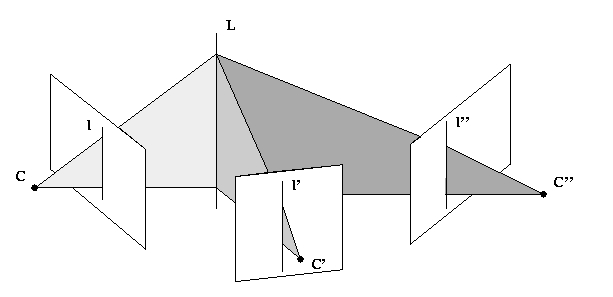
\includegraphics[width=80mm]{figures/threeviews.jpg}
  \caption{Trifocal geometry of three views}
  \label{fig:threeviews}
\end{figure}

$\mathcal{T}$ is then the trifocal tensor relating the 3 views together. It has 27 elements. There are 26 independent rations apart from the common overall scaling factor of the tensor. However, the tensor has only 18 independent parameters. Each of the three camera projection matrices has 11 parameters which makes $33$ in total. However, $15$ parameters must be subtracted to account for the projective world frame, thus leaving 18 parameters.

Since the trifocal tensor embeds the geometry of the three cameras in the scene, this implies that the camera matrices may be computed from the trifocal tensor up to a projective ambiguity~\cite{Hartley2004}. First, the epipoles $e^{\prime},e^{\prime \prime}$ are retrieved. Let $u_i$ and $v_i$ be the left and right null-vectors respectively of $\mathcal{T}_{i}$, \textit{i.e.:} $u_{i}^{T} \mathcal{T}_{i} = {\bf 0}^{T}, \mathcal{T}_{i}v_i = 0$. Then the epipoles are obtained as the null vectors of the following $ 3 \times 3$ matrices:
\begin{equation}
  e^{\prime T} [u_1, u_2, u_3] = 0  \text{ and } e^{\prime \prime T}[v_1, v_2, v_3] = 0
  \label{eq:recoveringepipoles}
\end{equation}
Next, to retrieve the camera matrices $P^{\prime}, P^{\prime \prime}$, the epipoles are first normalized to unit norm, and we have:
\begin{equation}
\begin{gathered}
  P^{\prime} = [[\mathcal{T}_{1}, \mathcal{T}_{2},\mathcal{T}_{3}] e^{\prime \prime} | e^{\prime}] \text{ and }\\ P^{\prime \prime} = [(e^{\prime \prime} e^{\prime \prime T} - I)[\mathcal{T}_{1}^{T}, \mathcal{T}_{2}^{T},\mathcal{T}_{3}^{T}] e^{\prime} | e^{\prime \prime}]
  \end{gathered}\label{eq:recoveringprojectionmatrices}
\end{equation}
The trifocal tensor can be computed from feature correspondences across the three views. Computation of tensor using correspondences of points or lines has been studied extensively in literature. The main linear algorithm presented by \texttt{Hartley}\cite{Hartley2004} is the straightforward method to compute the tensor. Other methods make use of \texttt{RANSAC} (RANdom SAmple Consensus) to enable the tensor estimation to be robust to outliers that usually cause the linear algebraic method to fail \cite{torr1997robust}.
Each triplet of corresponding image points gives 4 equations linearly independent. Therefore, a minimum set of 7 correspondences of non-planar points are needed for the trifocal tensor computation to uniquely determine the 27 entries of the tensor matrix. This method suffers from two issues however: the tensor is parameterized by all its entries and this does not take into account the tensor geometrical constraints, therefore, there is always a risk of obtaining an invalid tensor; and, using all available point correspondences causes the tensor to be significantly affected by the presence of strong outliers.
Hence, an algebraic minimization is needed there after, to use the linear solution as an initial estimate and re-parameterize it by the 24 entries of the projection matrices $P^\prime$ and $P^{\prime \prime}$. The desired tensor is found by minimizing the residual error. The latter algorithm leads to a geometrically valid tensor. However, the main weakness of the algebraic minimization method is that all point correspondences are involved in the tensor computation and still suffers from outliers in practice.
%%%%%%%%%%%%%%%%%%%%%%%%%%%%%%%%%%%%%%%%%%%%%%%%%%%%%%%%%%%%%%%%%%%%%%%%%%%%%%%%%%%%%%%%%%%%%%
\subsection{Visual Servoing}
Visual Servoing refers to the family of closed loop control techniques to control the degrees of freedom of an actuated system with visual feedback\cite{chaumette2006visual}. The vision data may be acquired from a camera that is mounted directly on the robot, or the camera can be fixed in the workspace so that it can observe the robot motion from a stationary configuration. The goal of many robotic applications is to place the robot at a desired configuration to manipulate an object in the environment. The objective of closed loop control techniques is to minimize an error function $e(t)$ defined as
\begin{equation}
  e(t) = s(t) - s^{*}
  \label{eq:servo1}
\end{equation}
where $s$ is a vector of visual features, and the vector $s^*$ has the desired values of these features at the desired configuration.

Then, to design the control scheme, the relationship between the time variation of the features $s$ and the camera velocity has to be found. Noting the spatial velocity of the camera $u_c = (v_c, \omega_c)$, where $v_c$ is the instantaneous linear velocity of the origin of the camera frame, and $\omega_c$ is the instantaneous angular velocity of the camera frame. The relationship between $\dot{s}$ and $u_c$ is given by
\begin{equation}
  \dot{s} = L_s u_c
  \label{eq:servo2}
\end{equation}
where $L_s$ is called the \textbf{interaction matrix} related to $s$. This matrix relates the rate of changes of the image feature velocities $\dot{s}$ to the rate of change of the pose parameters which is the camera velocity. From~\eqref{eq:servo1} and~\eqref{eq:servo2}, the relationship between the camera velocity and the derivative of the error is
\begin{equation}
  \dot{e} = L_s u_c
\label{eq:servo3}
\end{equation}
Considering $u_c$ as the input to the robot controller, to ensure an exponential decoupled decrease of the error, we would like to have $\dot{e} = -\lambda e$, using~\eqref{eq:servo3} we obtain the following control law equation
\begin{equation}
  u_c = -\lambda L_{s}^{+} e
\label{eq:servo4}
\end{equation}
where $L_{s}^{+}$ is the pseudo-inverse of $L_s$. This is the basic visual servoing closed loop system framework. Different visual servoing approaches differ only in the selection of the visual features $s$ and deriving their corresponding interaction matrices $L_s$.

There are three main classes of visual servoing: Image-based Visual Servoing (IBVS), Pose-based Visual Servoing (PBVS), and Hybrid Visual Servoing (HVS) \cite{chaumette2006visual}\cite{chaumette2007visual}. In IBVS, the features are computed from the 2D image data, while in PBVS, the features are computed from the estimated pose from image measurements. HVS use a combination of 2D and 3D visual features. The choice of the visual features is important and generally affects the performance of the visual servoing system. The IBVS approach is more robust to modeling and measurement noise than PBVS. However, the IBVS approach only guarantees local asymptotic stability. It also suffers from degenerate cases and may fail to reach the goal state. PBVS approach ensure global asymptotic stability if the pose estimation is perfect. The pose estimation algorithm must be realized in real-time to calculate the error at every control iteration, and hence more computationally expensive than IBVS approach. However, PBVS approach is more sensitive to image measurement noise and outliers. It usually also requires full knowledge of the geometric object model, and the camera intrinsic calibration.
%%%%%%%%%%%%%%%%%%%%%%%%%%%%%%%%%%%%%%%%%%%%%%%%%%%%%%%%%%%%%%%%%%%%%%%%%%%%%%%%%%%%%%%%%%%%%%
